\label{chap:RelationalModel}Neste capítulo, é feito uma análise detalhada com relação a base
relacional utilizada no modelo da \emph{\databaseName{}} e as regras de negócios envolvidas. 

Num primeiro momento, é descrito o cenário de negócios da sorveteria e num segundo explica-se o modelo
relacional vigente, suas entidades e as relações entre elas.

\section{Regras de Negócio}
\label{section:BusinessRules}
Nesta seção é  discutida as principais regras de negócio de interesse e o cenário das mesmas.

A rede de sorveteria Sweet possui 4 lojas, espalhadas pela cidade de São Paulo. As lojas possuem administrações distintas e dono único. As diferentes unidades podem ser observadas na tabela \ref{table:StoreUnits}.

\begin{center}
  \begin{table}[h]
\begin{centering}
\begin{tabular}{c|c|c}
\hline 
Unidade & Localização & Tamanho\tabularnewline
\hline 
1 & Shopping Morumbi & Grande\tabularnewline
\hline 
2 & Avenida Paulista & Pequena\tabularnewline
\hline 
3 & Berrini & Média\tabularnewline
\hline 
4 & Shopping Itaquera & Pequena\tabularnewline
\hline 
\end{tabular}
\par\end{centering}
\caption{\label{table:StoreUnits} Lojas físicas da \storeName{}, todas na cidade de São Paulo, SP.}
\end{table}
\vspace*{-40pt}
\par\end{center}

Numa compra nesta \emph{loja}, o \emph{cliente} dirige-se até uma das unidades da tabela \ref{table:StoreUnits}, escolhe o \emph{produto}, dado seu \emph{sabor}, o tipo de \emph{embalagem} e procede até o caixa, onde cada compra efetuada por um cliente deve gerar uma nota fiscal. Essa compra deve conter pelo menos uma unidade de sorvete. 

Sazonalmente, a franquia promove campanhas publicitárias e de códigos de \emph{cupons de desconto} e outras \emph{promoções} afim de aumentar o movimento, quantidade de vendas e a lucratividade geral das lojas franquiadas.

\section{Modelo relacional}

O modelo relacional, da figura \ref{figure:RelationalModel}, inclui as entidades \emph{Loja, Produto, Embalagem, Cliente}, presentes no cenário de negócio da seção \ref{section:BusinessRules}. Nesta seção analisa-se essas e outras entidades do modelo.

% A small example on how to use the "rotating" package.
%  Displays a figure and it's caption in landscape
\begin{landscape}
\begin{figure}[ht]
\begin{centering}
    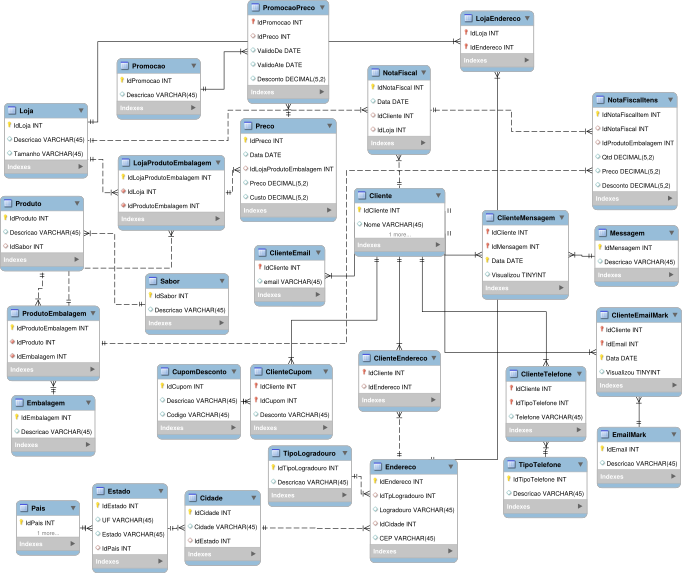
\includegraphics[width=1\textwidth]{RelationalModel}
    \caption{Modelo de base de dados relacional para a \storeFullName{}.}
    \label{figure:RelationalModel}
\end{centering}
\end{figure}
\end{landscape}

\section {Entidades}

Nesta seção, divide-se as entidades em \emph{fortes, fracas e associativas}. O objetivo dessa divisão é começar-se a entender quais são candidatas a serem chaves no modelo dimensional a ser utilizado.

\subsection{Entidades Fortes}
São as entidades que possuem chaves primárias independentes, e seus atributos podem ser unicamente identificados por ela. No modelo relacional da figura \ref{figure:RelationalModel}, são entidades fortes:

\begin{itemize}
\item \emph{Loja}: Define uma unidade da \storeFullName{}.
\item \emph{Produto}: Um produto da sorveteria. Ex: sorvete de chocolate.
\item \emph{Embalagem}: A embalagem de venda, com tamanho específico.
\item \emph{Cliente}: Informações a respeito do cliente da loja.
\end{itemize}

\subsection{Entidades Fracas}

É uma entidade cujos atributos não podem ser unicamente identificados sozinhos, portanto precisa de uma chave estrangeira ao menos para que isso aconteça. 

\begin{itemize}
\item \emph{Promocao}: Uma promoção sazonal da franquia.
\item \emph{CupomDesconto}: Um cupom de desconto específico.
\item \emph{TipoTelefone}: Telefone com DDD.
\item \emph{Sabor}: Um sabor de de sorvete.
\item \emph{EmailMark}: Endereço de e-mail.
\item \emph{Mensagem}: Uma mensagem enviada a um e-mail.
\item \emph{Endereco}: Endereço único (localidade).
\item \emph{TipoLogradouro}: Identifica o tipo de logradouro.
\item \emph{Cidade}: Identificação da cidade.
\item \emph{Estado}: Identificação do estado.
\item \emph{Pais}: Identificação do país.
\end{itemize}

\subsection{Entidades Associativas}

Uma entidade associativa é um termo de modelagem relacional que significa uma relação de muitos para muitos a nível de entidades e relações. As tabelas desse tipo são denominadas \emph{associativas}.

\begin{itemize}
\item \emph{ProdutoEmbalagem}: Relação entre Produto e Embalagem.
\item \emph{LojaProdutoEmbalagem}: Relação entre Loja e Produto com Embalagem.
\item \emph{Preco}: Associa um valor fiat a um produto.
\item \emph{NotaFiscal}: Relatório de venda de produto(s).
\item \emph{NotaFiscalItens}: O relatório de um item de venda.
\item \emph{PromocaoPreco}: Preço referente a uma promoção específica.
\item \emph{ClienteCupom}: Cupom de um cliente.
\item \emph{ClienteEmail}: E-mail de um cliente.
\item \emph{ClienteEndereco}: Endereço de um  cliente.
\item \emph{ClienteTelefone}: Telefone de um cliente.
\item \emph{LojaEndereco}: Endereço de uma loja.
\item \emph{ClienteEmailMark}: Visualização ou não de um determinado e-mail por parte do cliente.
\item \emph{ClienteMensagem}: Mensagem enviada ao cliente por e-mail.
\end{itemize}

\section{Dores do Negócio}

O objetivo da modelagem dimensional a ser feita é responder os seguintes questionamentos:

\begin{enumerate}
\item Questões de Negócio/Analíticas
\item Quais são as lojas mais lucrativas?
\item Quais são os clientes que mais compram?
\item Quais promoções surtiram mais efeito?
\item Quais produtos mais vendem?
\end{enumerate}

Por isso, o modelo dimensional deverá ter como \emph{fato} principal a tabela \emph{Vendas}.
